\documentclass[../main]{subfiles}
\bibliography{reference, reference_web}
\graphicspath{{../figures/}}

\begin{document}


% 図表の例:コーンペネトロメータを\reffig{fig:cone_penetrometer}に示す.
% \reftab{tab:traffic_cone_index}が示すように,各建設機械の走行に必要とされているコーン指数は既にわかっている.

\section{背景}
\label{sec:intro_background}
\subsection{石油精製プラント点検の現状}
\label{sec:intro_plant_current}


近年,地球温暖化の進行を抑えるため,カーボンニュートラルの実現が求められている.
しかし,\reffig{fig:oil_consumption}に示されるように,石油をはじめとする化石燃料は,将来的にもエネルギー源として重要な役割を果たすと予想されている.\cite{ritchie2023energy}

石油の精製は,ガソリン,ディーゼル燃料,ジェット燃料などの輸送用エネルギー資源だけでなく,プラスチック,化学肥料,医薬品,合成繊維など,幅広い化学製品を生み出すために欠かせない工程である.その中心的役割を担うのが,\reffig{fig:view_plant}に示す石油精製プラントであり,そこにはポンプ,熱交換器,蒸留装置,配管など多種多様な装置が複雑に組み合わさっている.\cite{eneos2024,Shvindin2008A}
これらの装置が適切に稼働することで,高品質なプロダクトが安定して供給され,産業や社会の基盤を支えている.

一方,保守作業はどの産業においても重要な要素であり,石油精製プラントも例外ではない.
設備は老朽化や環境条件による劣化で故障することがあり,その結果,操業停止による生産遅延,修理費の増加などの損失が発生する.
さらに,石油精製プラントでは可燃性物質を多数扱うため,他の産業施設に比べて火災や爆発など重大な事故が発生するリスクが高く,その被害は甚大になり得る.\cite{Tang2021}
こうしたリスクを低減するためには,設備の異常を早期に発見し,適切な対策を講じることが求められる.

現状では,プラント内の設備点検は専属の現場作業員が定期的な巡回で行い,視覚・聴覚・嗅覚・触覚による異常の有無の確認が基本である.
こうした点検は1日に4~5回実施され,昼夜を問わず行われているため,夜間作業による負担や,高齢化による熟練人材の不足,熟練度の差による点検品質のばらつきといった様々な課題が生じている.
これらの理由から,プラント内点検の自動化が求められている.

\begin{figure}[t]
  \centering
  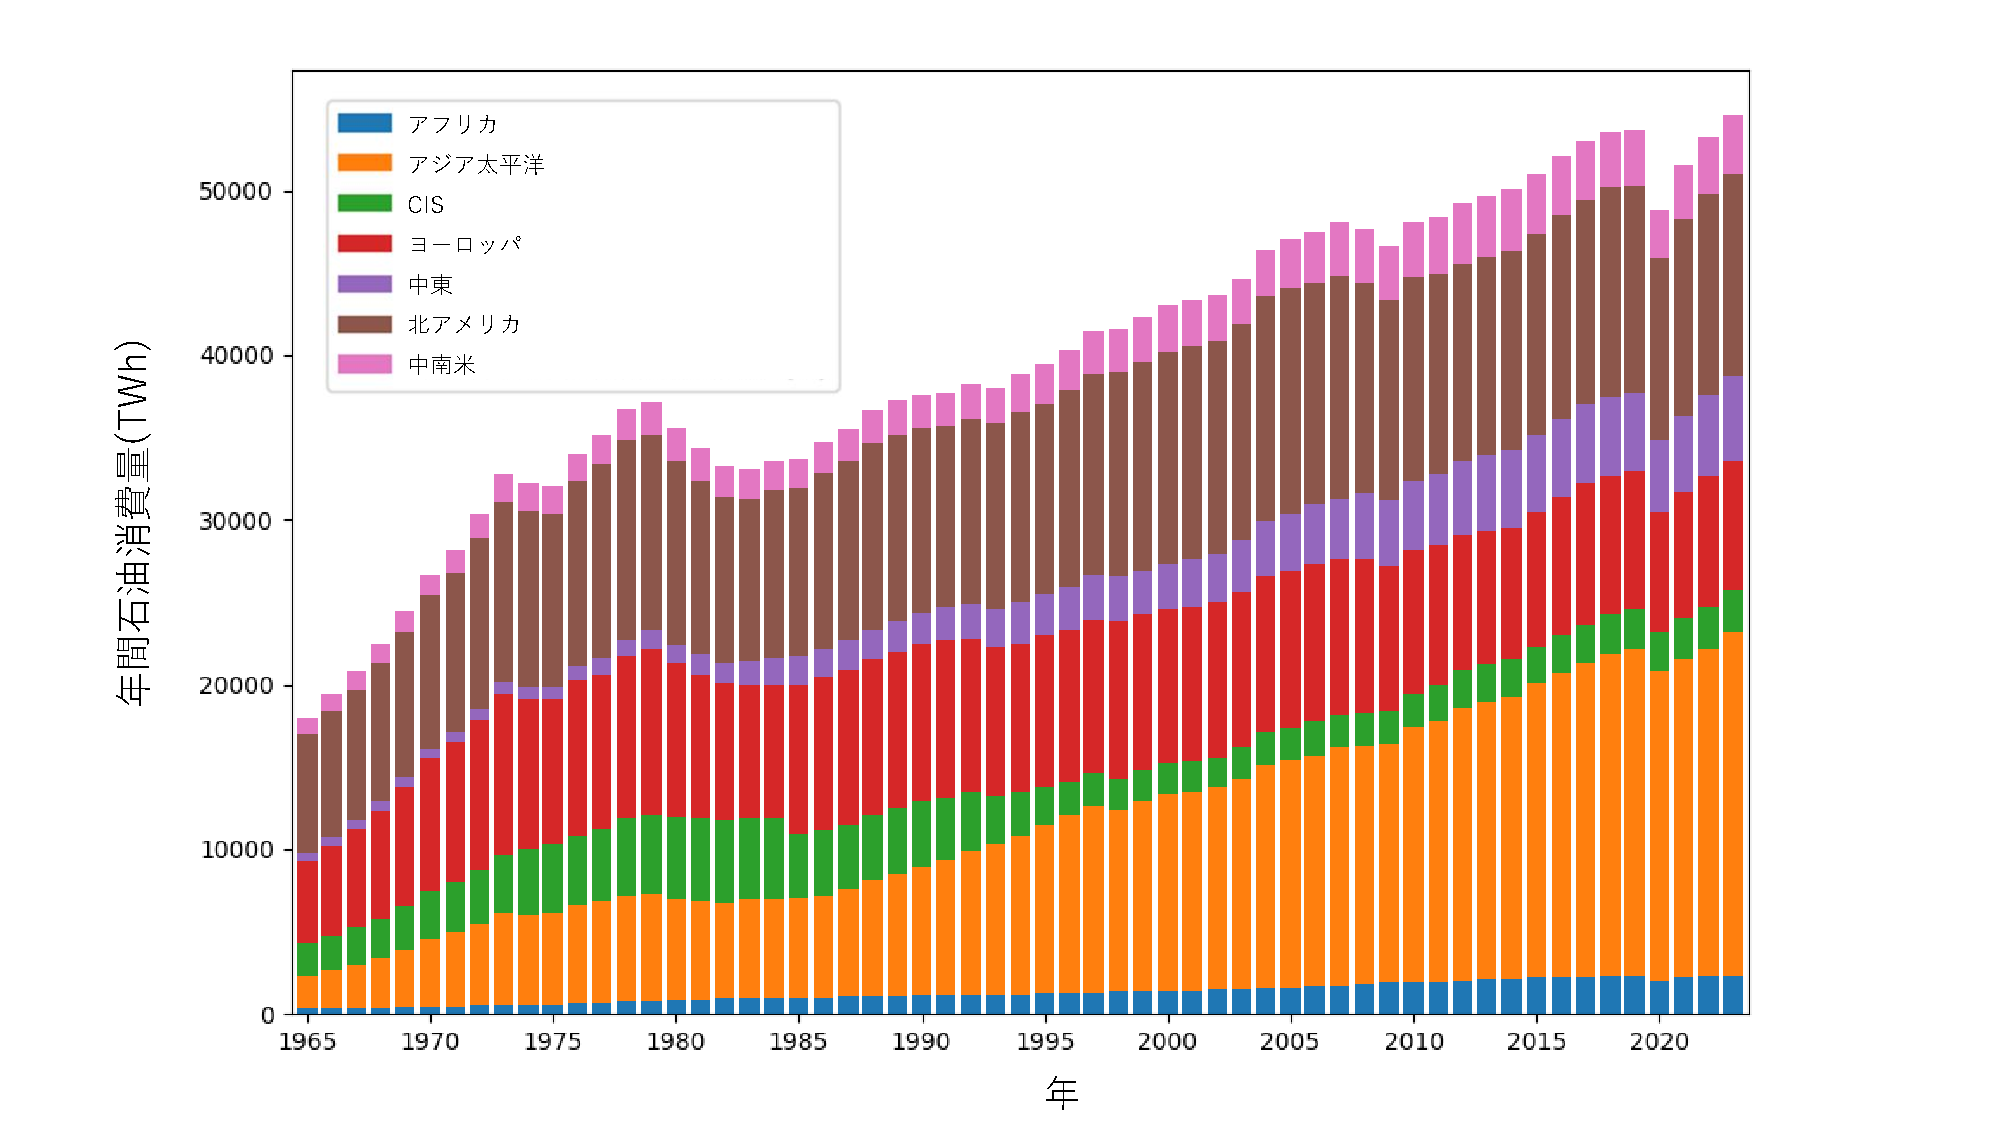
\includegraphics[keepaspectratio, width=0.5\linewidth]{chap1/oil_consumption.pdf}
  \caption{世界石油消費量の推移}
  \label{fig:oil_consumption}
\end{figure}

\begin{figure}[t]
  \centering
  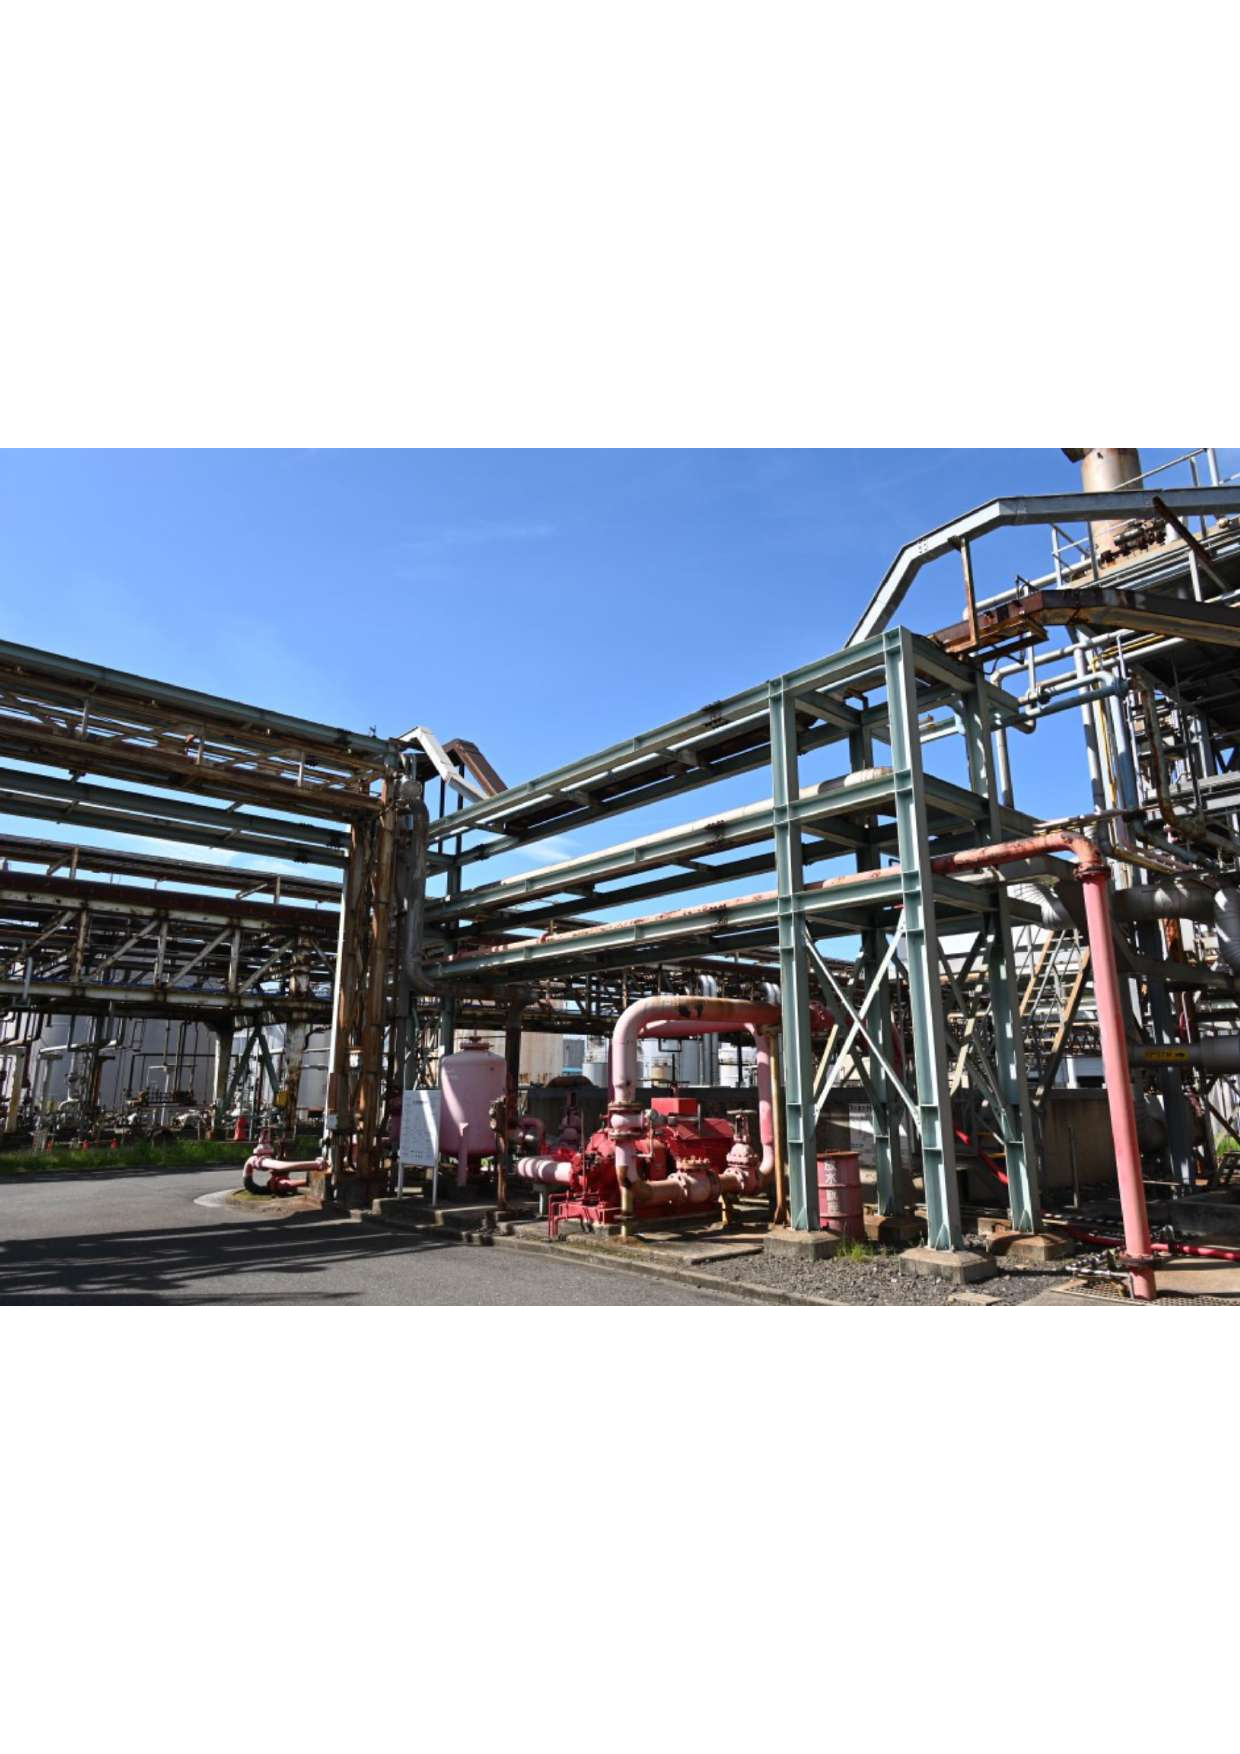
\includegraphics[keepaspectratio, width=0.5\linewidth]{chap1/view_plant.pdf}
  \caption{石油精製プラント}
  \label{fig:view_plant}
\end{figure}


\begin{table}[t]
  \caption{プラント内の異常の種類(株式会社ENEOSより提供)}
  \label{tab:plant_anomalies}
  \centering
  \begin{tabular}{lll}
    \toprule
    対象機器 & 監視対象 & 検査手法 \\
    \midrule
    \textbf{ポンプの異常} & ベアリング異音 & 聴覚 \\
                 & 漏洩による白煙発生 & 視覚、嗅覚 \\
                 & 漏洩による着火 & 視覚、嗅覚 \\
                 & オイラーのオイルレベル低下 & 視覚 \\
                 & 閉塞等による冷却水低下、喪失 & 触覚 \\
                 & 発熱 & 触覚 \\
    \midrule
    \textbf{配管異常} & 外面腐食の進行 & 視覚 \\
               & 保温板金の劣化 & 視覚 \\
               & 保温劣化による表面温度上昇 & 触覚 \\
               & 腐食によるガス・油漏洩 & 視覚、嗅覚 \\
               & フランジ部からのガス・油漏洩 & 視覚、嗅覚 \\
    \midrule
    \textbf{その他機器の異常} & 加熱炉の耐火煉瓦脱落による炉壁発熱 & 視覚 \\
                   & バルブの誤開閉 & 視覚 \\
    \midrule
    メータ読み込み & 圧力計、温度計等 & 視覚 \\
    \bottomrule
  \end{tabular}
\end{table}

\subsection{プラント内音響点検の特徴}
\label{sec:intro_plant_characteristics}

石油精製プラント内では,多様な装置が複雑に組み合わさり,その稼働状況によって各種の異常が発生し得る.
\reftab{tab:plant_anomalies}に示すように,プラント内ではポンプや配管,その他設備に関連した多種多様な異常が確認され,
それぞれの異常毎に適した人間の感覚による点検が行われている.

その中でも,ポンプはプラント内での液体やスラリー(液体と固体の混合物)の移動に用いられる装置であり,プラント内にて最も多く設置されている機器の一つである.
ポンプは内部に回転機構を有しており,その中核には流体を昇圧・輸送するための回転軸が配置されている.
回転軸の安定した回転を支えるため,ポンプ内部にはベアリングと呼ばれる部品が組み込まれている.
ベアリングは回転軸に掛かるラジアル(軸方向)およびスラスト(軸垂直方向)方向の加重を受け止め,摩擦を提言する役割を担う.

しかしながら,ポンプが長時間稼働を続ける中で,ベアリングは次第に摩耗し,その性能を劣化させていく.
ベアリングの摩耗が進行すると,騒音や異常な温度上昇が起こるだけでなく,軸の振れ周りの振動が大きくなり,
ポンプ全体の異常停止や,ポンプの破損につながる可能性がある.
特に石油精製プラントのような安定操業が求められる現場では,ポンプ内のベアリング摩耗は極力未然に防止検知することが重要である.

ベアリング摩耗の検知の一例として,振動系を用いた検知があげられる.
ベアリングの摩耗が進行すると,軸の振れ周りの振動が大きくなるため,振動センサを用いてベアリングの振動を計測し,異常を検知することが可能である.

その中でも,本研究では聴覚による点検に着目する.
聴覚による異常検知は点検において重要な意義がある.
というのも,音響信号は空気を媒体として伝搬するため,視覚や触覚と異なり,遠方の異常音を検知することが可能である.
したがって,本研究では聴覚による点検を実施するために,マイクロフォンを用いた音響点検に焦点を当てる.

\end{document}
